%---------------------------------------------------------------------------
%    Portada en tiks
%---------------------------------------------------------------------------

\begin{tikzpicture}[remember picture,overlay]
	\coordinate (title) at ($(current page.north)+(0,-25mm)+(0,10mm)$);
	\coordinate (tituba) at ($(current page.south)+(0,25mm)$);
	
	%	Poner la imagen de fondo
%	\node[inner sep=0pt,opacity=0.03] at ($(current page.center)+(0,2mm)$) {\includegraphics[height=0.95\paperheight]{anexos/img-portada_Bunny.png}};
	
	%	Poner la imagen en el espacio sobrante
%	\node[inner sep=0pt,anchor=south,opacity=0.5] at ([shift={(0,30mm)}]tituba) {\includegraphics[height=80mm]{anexos/img-portada_Bunny.png}};
	
	\node[inner sep=0pt,anchor=north] at (title) {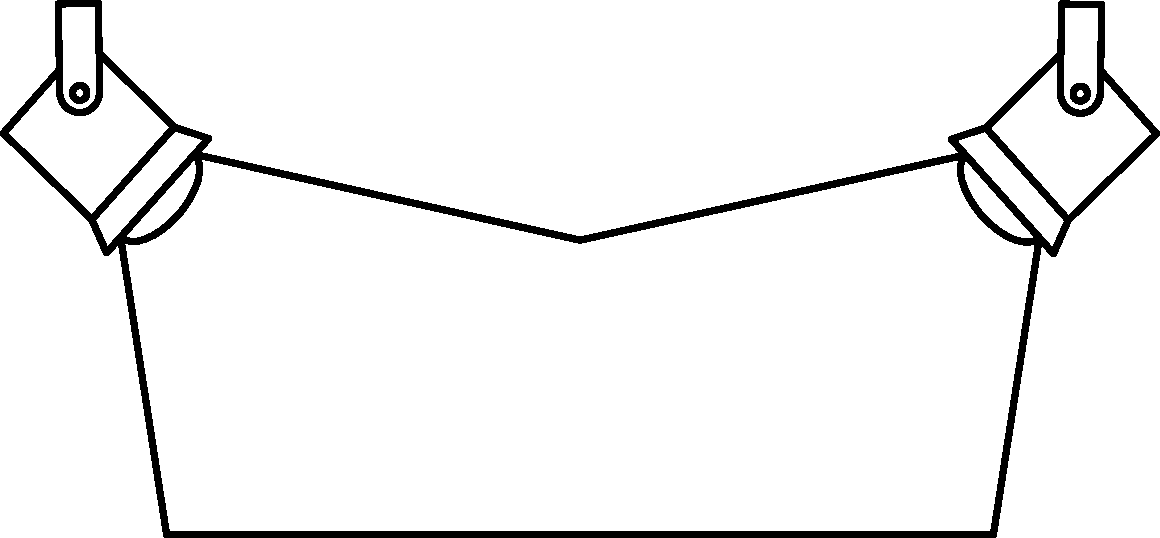
\includegraphics{LaTeX_PilarPlayscript/vector-portada_Marco_luces.pdf}};
	
	\node[inner sep=0pt,anchor=north] at ([shift={(0,-40mm)}]title) {
		\begin{minipage}[m][50mm]{140mm}
			\setlength{\parskip}{6pt}
			\centering
			
			{\fontsize{35}{40}\selectfont \rmfamily \bfseries\itshape \encabezado}
			
			{\fontsize{16}{18}\selectfont \rmfamily \scshape \subencabezado}
			
			\vspace{8pt}
			
			{\fontsize{14}{14}\selectfont \emph{De:} \dramaturgo}
		\end{minipage}
	};
	
	\node[inner sep=0pt,anchor=north] at ([shift={(0,-100mm)}]title) {
		\begin{minipage}{140mm}
			\setlength{\parskip}{4pt}
			\centering
			\fontsize{15}{16}\selectfont
			
			Dirección: \director
			
			Técnico de escena: \technician
			
			\vspace{8pt}
			
			\texttt{Rev. \fecha}
			
		\end{minipage}
	};
	
	\node[inner sep=0pt,anchor=south] at (tituba) {
\includegraphics[height=20mm]{LaTeX_PilarPlayscript/vector-TITUBA_Expand_1inkB.pdf}};
\end{tikzpicture}
